%-----------------------------------------------%
%             filename: skeleton.tex
%-----------------------------------------------%
\documentclass[aps,twocolumn]{revtex4-1}
\usepackage{graphicx}
\usepackage{ifpdf}
\ifpdf
	\usepackage[backref]{hyperref}
	%\usepackage[backref,pageanchor=true,plainpages=false, pdfpagelabels,bookmarks,bookmarksnumbered]	{hyperref}
\else
\fi

\usepackage{crs}

% see http://goo.gl/5Fo27
\newtoggle{thmsty}
\toggletrue{thmsty}
%\togglefalse{thmsty}

% see http://goo.gl/7jLZ9
\makeatletter
\newlength \figwidth
\if@twocolumn
  \setlength \figwidth {0.8\columnwidth}
\else
  \setlength \figwidth {0.5\textwidth}
\fi
\makeatother

\begin{document} 

\title{\bf Intrinsic information representation in biological systems}

\author{a1$^{1}$, a2$^{1}$, a3$^{1}$, a4$^{1,2,3}$}

\affiliation{$^1$Department of Systems and Computational Biology,\\ $^2$Dominick P. Purpura Department of Neuroscience, \\ $^3$Department of Pathology, Albert Einstein College of Medicine, 1301 Morris Park Ave, Bronx, NY 10461, USA}

\date{\today}
\begin{abstract}
One of the most important aspects of advancing theory in biology is the development of a constructed language that can be explicitly and precisely defined and supports communication among scientists, between scientists and computers, and even within individual scientists themselves. Such a language should itself be evolvable and support flexible abstractions that enable the unification and compression of redundant information. It would be useful for such a language to be formally specified prior to or in concert with the development of a computational implementation that may support complementary organization of semi-autonomously linked and computable data. We propose the adaptation of a language originally developed in a mathematical context that apparently meets these criteria. We argue for the particular choice we suggest, not from a mathematical perspective but, by providing an example of the way in which this language enables precise qualitative reasoning and flexible methods of abstraction with respect to integrating biological information in a manner that would, ideally, be analogous to the way in which information is integrated by biological systems themselves. Enabling lossless compression and representation of synthetic knowledge about biological systems, in addition to raw biological data, is necessary for understanding in the context of limited cognitive and other computational resources.
\end{abstract}

\maketitle

\tableofcontents

\section{Introduction}
The development of a formal language for modeling biological systems was suggested by Joseph Woodger in collaboration with the developmental biologist Conrad Waddington and the logician Alfred Tarski as early as 1937 \cite{Woodger1937,Woodger1951,Woodger1952,Woodger1952a}. At that time it was perhaps difficult to understand how such a language could be put to use. Today we have tools that could enable the use of such a language: namely 1) computational machines to automate the details of routine transformations within the language and 2) large, accessible, growing repositories of biological data. Though we have access to necessary infrastructure, we lack such a language suggested by Woodger and others throughout the course of the 20th century as we have continued to rely on natural language heuristics to communicate and reason about biological systems.

Category theory \cite{Lane1985,Lane1998,MacLane1992,Lawvere1997,Lawvere2003,Awodey2006} is a language that has been suggested since Woodger to provide a framework for representing and reasoning about biological systems \cite{GOGUEN1979,Ehresmann2007,Louie2009}. What is immediately useful about this language from the perspective of biology is that it presents as primitive the notion of transformation or interaction between objects. In fact, from this point of view, a defining characteristic of any entity (e.g. a protein, cell, organism, or population) is structural: the set of relationships between it and other entities under consideration. Intrinsic properties are taken into account implicitly in this framework since the possible set of relationships between any object and any other is constrained by the nature of its intrinsic properties. 

What is less obvious at first meeting is the way in which category theory, especially with regard to its interface with logic and geometry \cite{MacLane1992,Jacobs1998}, enables the precise definition of what might be viewed as a framework for explaining the nature and development of so-called \emph{emergent properties} of systems of interacting processes. This expression is general enough that it can be equally well applied to the consideration of relationships between any levels of biological organization and may be generalizable to arbitrary physical contexts. This unity deriving from the judicious definition of underlying categorical concepts along the way is precisely the type of abstraction that we argue is necessary to enable compression without loss of biological information and thus synthesis of existing biological knowledge.

Here we define the concepts from category theory necessary to understand the way in which interacting objects at one level of organization (e.g. molecules) can produce phenomena that would themselves be identifiable as derived objects (e.g. cells) that justify the very conceptualization of a \emph{level of organization} in the first instance. Here we focus exclusively on defining the boundary conditions relating levels (e.g. molecules and cells or cells and multicellular organisms) of organization, which are necessary to understand in the course of defining a dynamical system that could model the \emph{evolution} of such. What results is a refinement of the concept of the levels of organization that are ubiquitously employed in biology and examples of which are used so far only heuristically as guides to pre-existing intuition. Understanding how to integrate information regarding biological processes across such levels of organization is fundamental to the understanding of complex phenotypes and the associated set of contingencies necessary to account for in methods that may be targeted at controlling or otherwise manipulating them.

[ Note that biological systems are concretely represented as graphs of some kind and all the letters representing categories can be specialized to categories of graphs of some kind ]

\section{Biological information}
\subsection{System-environment duality}
Distinction between biological systems or some components thereof and the environments within which they are embedded is implied in models of such systems. This distinction is useful in many contexts, but the boundary between a biological system and its environment is dependent upon the level of resolution of the \emph{model and modeler} independent of its relationship to properties of the biological system itself \cite{Fontana1996}. In this light, it is desirable to develop a model of biological systems that supports variation of this boundary without requiring complete reconfiguration of the model. Constructing a framework for such models requires the determination, unification, and incorporation of abstract features of biological systems that are invariant across levels of organization from molecules to cells, organisms, populations, communities, ecosystems and more fine-grained levels of resolution that likely lie between these broadly and imprecisely defined perspectives one can take with regard to representing biological systems.


\subsection{Transformation of biological information at system-environment boundaries}
The use of categorical adjunctions to model intrinsic information representation in biological systems has been suggested \cite{GOGUEN1979,Ellerman2005}, but these efforts have yet to be incorporated into more detailed theories. This may be in part a result of the difficulty in specifying the appropriate level of abstraction at which a precise metaphor can be developed between collections of interacting biological entities and a particular type of mathematical structure. We begin here by developing the prerequisite definitions to explain why the transformation of biological information is naturally represented as a pair of adjoint functors in the context of category theory. A relevant piece of intuition to associate to what follows is that any interaction between biological entities is, minimally, a dyadic relationship wherein contingencies associated to other interactions of each of the participants establishes prerequisite potential value to high fidelity transmission and representation of information regarding the state of other collections of spatio-temporally distant interactions. The participants in such a dyadic interaction are modelled as categories because each may represent an underlying arbitrarily complicated collection of interactions that are necessary for the very existence of the interface implicit to any interaction.

\iftoggle{thmsty}{
\begin{definition}
\label{definition-category}
}{}
A {\it category} $\mathcal{C}$ is:
\begin{enumerate}
\item A set of objects $\Ob(\mathcal{C})$.
\item For each pair $x, y \in \Ob(\mathcal{C})$ a set of morphisms
$\Mor_\mathcal{C}(x, y)$.
\item For each triple $x, y, z\in \Ob(\mathcal{C})$ a composition
map $ \Mor_\mathcal{C}(y, z) \times \Mor_\mathcal{C}(x, y)
\to \Mor_\mathcal{C}(x, z) $, denoted $(\phi, \psi) \mapsto
\phi \circ \psi$.
\end{enumerate}
Such that these constraints are satisfied:
\begin{enumerate}
\item For every element $x\in \Ob(\mathcal{C})$ there exists a
morphism $\text{id}_x\in \Mor_\mathcal{C}(x, x)$ such that
$\text{id}_x \circ \phi = \phi$ and $\psi \circ \text{id}_x = \psi $.
\item Composition is associative, i.e., $(\phi \circ \psi) \circ \chi =
\phi \circ ( \psi \circ \chi)$.
\end{enumerate}
\iftoggle{thmsty}{
\end{definition}
}

\iftoggle{thmsty}{
\begin{definition}
\label{definition-functor}
}{}
A {\it functor} $F : \mathcal{A} \to \mathcal{B}$
between two categories $\mathcal{A}, \mathcal{B}$ is:
\begin{enumerate}
\item A map $F : \Ob(\mathcal{A}) \to \Ob(\mathcal{B})$.
\item For every $x, y \in \Ob(\mathcal{A})$ a map
$F : \Mor_\mathcal{A}(x, y) \to \Mor_\mathcal{B}(F(x), F(y))$,
denoted $\phi \mapsto F(\phi)$.
\end{enumerate}
These data should be compatible with composition and identity morphisms
in the following manner: $F(\phi \circ \psi) =
F(\phi) \circ F(\psi)$ for a composable pair $(\phi, \psi)$ of
morphisms of $\mathcal{A}$ and $F(\text{id}_x) = \text{id}_{F(x)}$.
\iftoggle{thmsty}{
\end{definition}
}

\iftoggle{thmsty}{
\begin{definition}
\label{definition-transformation-functors}
}{}
Let $F, G : \mathcal{A} \to \mathcal{B}$ be functors.
A {\it natural transformation}, or a {\it morphism of functors}
$t : F \to G$, is a collection $\{t_x\}_{x\in \Ob(\mathcal{A})}$
such that
\begin{enumerate}
\item $t_x : F(x) \to G(x)$ is a morphism in the category $\mathcal{B}$, and
\item for every morphism $\phi : x \to y$ of $\mathcal{A}$ the following
diagram is commutative
$$
\xymatrix{
F(x) \ar[r]^{t_x} \ar[d]_{F(\phi)} & G(x) \ar[d]^{G(\phi)} \\
F(y) \ar[r]^{t_y} & G(y) }
$$
\end{enumerate}
\iftoggle{thmsty}{
\end{definition}
}

We can define a category having functors as objects and natural transformations as morphisms, which is called a functor category, by recognizing that every functor $F$ comes with the {\it identity} transformation $\text{id}_F : F \to F$. In addition, given a morphism of
functors $t : F \to G$ and a morphism of functors $s : E \to F$
then the {\it composition} $t \circ s$ is defined by the rule
$$
(t \circ s)_x = t_x \circ s_x : E(x) \to G(x)
$$
for $x \in \Ob(\mathcal{A})$.
This is a morphism of functors
from $E$ to $G$.
Thus, given categories
$\mathcal{A}$ and $\mathcal{B}$ we obtain the category of functors between $\mathcal{A}$ and
$\mathcal{B}$.

\iftoggle{thmsty}{
\begin{definition}
\label{definition-equivalence-categories}
}{}
An {\it equivalence of categories}
$F : \mathcal{A} \to \mathcal{B}$ is a functor such that there
exists a functor $G : \mathcal{B} \to \mathcal{A}$ such that
the compositions $F \circ G$ and $G \circ F$ are isomorphic to the
identity functors $\text{id}_\mathcal{B}$,
respectively $\text{id}_\mathcal{A}$.
In this case we say that $G$ is a {\it quasi-inverse} to $F$.
\iftoggle{thmsty}{
\end{definition}
}

\iftoggle{thmsty}{
\begin{definition}
\label{definition-adjoint}
}{}
Let $\mathcal{C}$, $\mathcal{D}$ be categories.
Let $u : \mathcal{C} \to \mathcal{D}$ and
$v : \mathcal{D} \to \mathcal{C}$ be functors.
We say that $u$ is a {\it left adjoint} of $v$ or that
$v$ is a {\it right adjoint} to $u$, written $u \dashv v$, if there are bijections
$$
\phi_{X,Y}:\Mor_\mathcal{D}(u(X), Y)
\simeq
\Mor_\mathcal{C}(X, v(Y))
$$
functorial in $X \in \Ob(\mathcal{C})$, and
$Y \in \Ob(\mathcal{D})$.
\iftoggle{thmsty}{
\end{definition}
}

Morphisms that are associated with each other according to the bijections of an adjunction are called {\it adjoint transposes} of one another. If $g:u(X) \rightarrow Y$, $g \in \Mor(\cD)$ then $g^*: X \rightarrow v(Y)$, $g^* \in \Mor(\cC)$ is given by $\phi_{X,Y}(g) = g^*$. Similarly for $f: X \rightarrow v(Y)$, $f \in \Mor(\cC)$ with $f^*:u(X) \rightarrow Y$, $f^* \in \Mor(\cD)$ is given by $\phi_{X,Y}^{-1}(f) = f^*$. We see then that $g^* = f$ and $f^* = g$.

\iftoggle{thmsty}{
\begin{definition}
\label{definition-opposite}
}{}
Given a category $\mathcal{C}$ the {\it opposite category}
$\mathcal{C}^{opp}$ is the category with the same objects
as $\mathcal{C}$ but all morphisms reversed.
\iftoggle{thmsty}{
\end{definition}
}

\iftoggle{thmsty}{
\begin{definition}
\label{definition-contravariant}
}{}
Let $\mathcal{C}$, $\mathcal{S}$ be categories.
A {\it contravariant} functor $F$
from $\mathcal{C}$ to $\mathcal{S}$
is a functor $\mathcal{C}^{opp}\to \mathcal{S}$.
\iftoggle{thmsty}{
\end{definition}
}

\iftoggle{thmsty}{
\begin{definition}
\label{definition-presheaf}
}{}
Let $\mathcal{C}$ be a category.
\begin{enumerate}
\item A {\it presheaf of sets on $\mathcal{C}$}
or simply a {\it presheaf} is a contravariant functor
$F$ from $\mathcal{C}$ to $\textit{Sets}$. When $F$ is a covariant functor $F : \mathcal{C}^{opp} \rightarrow \textit{Sets}$.
\item The category of presheaves is denoted $\textit{PSh}(\mathcal{C})$.
\end{enumerate}
\iftoggle{thmsty}{
\end{definition}
}

\iftoggle{thmsty}{
\begin{definition}
\label{definition-products}
}{}

Let $x, y\in \Ob(\mathcal{C})$,
A {\it product} of $x$ and $y$ is
an object $x \times y \in \Ob(\mathcal{C})$
together with morphisms
$p\in \Mor_{\mathcal C}(x \times y, x)$ and
$q\in\Mor_{\mathcal C}(x \times y, y)$ such
that the following universal property holds: for
any $w\in \Ob(\mathcal{C})$ and morphisms
$\alpha \in \Mor_{\mathcal C}(w, x)$ and
$\beta \in \Mor_\mathcal{C}(w, y)$
there is a unique
$\gamma\in \Mor_{\mathcal C}(w, x \times y)$ making
the diagram
$$
\xymatrix{
w \ar[rrrd]^\beta \ar@{-->}[rrd]_\gamma \ar[rrdd]_\alpha & & \\
& & x \times y \ar[d]_p \ar[r]_q & z \\
& & x &
}
$$
commute.
\iftoggle{thmsty}{
\end{definition}
}

\iftoggle{thmsty}{
\begin{definition}
\label{definition-has-products-of-pairs}
}{}
We say the category $\mathcal{C}$ {\it has products of pairs
of objects} if a product $x \times y$
exists for any $x, y \in \Ob(\mathcal{C})$.
\iftoggle{thmsty}{
\end{definition}
}

\iftoggle{thmsty}{
\begin{definition}
\label{definition-coproducts}
}{}
Let $x, y \in \Ob(\mathcal{C})$,
A {\it coproduct}, or {\it amalgamated sum} of $x$ and $y$ is
an object $x \amalg y \in \Ob(\mathcal{C})$
together with morphisms
$i \in \Mor_{\mathcal C}(x, x \amalg y)$ and
$j \in \Mor_{\mathcal C}(y, x \amalg y)$ such
that the following universal property holds: for
any $w \in \Ob(\mathcal{C})$ and morphisms
$\alpha \in \Mor_{\mathcal C}(x, w)$ and
$\beta \in \Mor_\mathcal{C}(y, w)$
there is a unique
$\gamma \in \Mor_{\mathcal C}(x \amalg y, w)$ making
the diagram
$$
\xymatrix{
& y \ar[d]^j \ar[rrdd]^\beta \\
x \ar[r]^i \ar[rrrd]_\alpha & x \amalg y \ar@{-->}[rrd]^\gamma \\
& & & w
}
$$
commute.
\iftoggle{thmsty}{
\end{definition}
}

\iftoggle{thmsty}{
\begin{definition}
\label{definition-has-coproducts-of-pairs}
}{}
We say the category $\mathcal{C}$ {\it has coproducts of pairs
of objects} if a coproduct $x \amalg y$
exists for any $x, y \in \Ob(\mathcal{C})$.
\iftoggle{thmsty}{
\end{definition}
}

\iftoggle{thmsty}{
\begin{definition}
\label{definition-product-category}
}{}
Let $\mathcal{A}$, $\mathcal{B}$ be categories.
The {\it product category} is the category
$\mathcal{A} \times \mathcal{B}$ with
objects
$\Ob(\mathcal{A} \times \mathcal{B}) =
\Ob(\mathcal{A}) \times \Ob(\mathcal{B})$
and
$$
\Mor_{\mathcal{A} \times \mathcal{B}}((x, y), (x', y'))
:=
\Mor_\mathcal{A}(x, x')\times
\Mor_\mathcal{B}(y, y').
$$
Composition of morphisms is defined according to components.
\iftoggle{thmsty}{
\end{definition}
}

\iftoggle{thmsty}{
\begin{definition}
\label{definition-bifunctor}
}{}
Given categories $\mathcal{C}_1$, $\mathcal{C}_2$, and $\mathcal{D}$. A {\it bifunctor} or binary functor or 2-ary functor or functor of two variables, $F$, is a functor whose domain is the product of two categories $F: \mathcal{C}_1 \times \mathcal{C}_2 \rightarrow \mathcal{D}$.
\iftoggle{thmsty}{
\end{definition}
}

\iftoggle{thmsty}{
\begin{definition}
\label{definition-hom-functor}
}{}
The {\it hom-functor} is a bifunctor defined on the product of a category $\mathcal{C}$ with its self-dual category $\mathcal{C}^{opp}$, which takes values in the category $\textit{Sets}$. Thus for a category $C$ its hom-functor is 
$$
hom(-,-): \mathcal{C}^{opp} \times \mathcal{C} \rightarrow \textit{Sets},
$$
which can be curried in two ways
\begin{eqnarray*}
hom^{(-)} &:& \mathcal{C}^{opp} \rightarrow \textit{Sets}^{\mathcal{C}},\\
hom_{(-)} &:& \mathcal{C} \rightarrow \textit{Sets}^{\mathcal{C}^{opp}}.
\end{eqnarray*}
The hom-functor maps
\begin{enumerate}
\item objects $(c,c') \in \mathcal{C}^{opp} \times \mathcal{C}$ to the hom-set $\Mor_{\mathcal{C}} (c,c')$, which is the set of morphisms in $\mathcal{C}$ with domain $c$ and codomain $c'$.
\item morphisms 
$$
(f,g):(c,c') \rightarrow (d,d') \in \Mor(\mathcal{C}^{opp} \times \mathcal{C}),
$$
where $f:d \rightarrow c \in \Mor(\mathcal{C})$ and $g:c' \rightarrow d' \in \Mor(\mathcal{C})$, to the set function
\begin{eqnarray*}
\Mor_{\mathcal{C}}(c,c') &\rightarrow& \Mor_{\mathcal{C}}(d,d')\\
(c \rightarrow c') &\mapsto& (d \rightarrow c \rightarrow c' \rightarrow d')
\end{eqnarray*}
\end{enumerate}
\iftoggle{thmsty}{
\end{definition}
}

\iftoggle{thmsty}{
\begin{definition}
\label{definition-representable-functor}
}{}
For a hom-functor $hom(-,-): \mathcal{C}^{opp} \times \mathcal{C} \rightarrow \textit{Sets}$ for $c \in \Ob(\mathcal{C})$ a covariant and contravariant functor can be derived by specializing the hom-functor to morphisms out of or into the object $c$ as
\begin{eqnarray*}
h^c \equiv hom(-,c) &:& \mathcal{C}^{opp} \rightarrow \textit{Sets}\\
h_c \equiv hom(c,-) &:& \mathcal{C} \rightarrow \textit{Sets}.
\end{eqnarray*}
Functors that are isomorphic to $h^c$ or $h_c$ are referred to as {\it corepresentable or representable functors} respectively and $c$ is their {\it representing object}. Note that $h^c \in \Ob(\textit{PSh}(\mathcal{C}))$.
\iftoggle{thmsty}{
\end{definition}
}{}

\begin{figure}
\noindent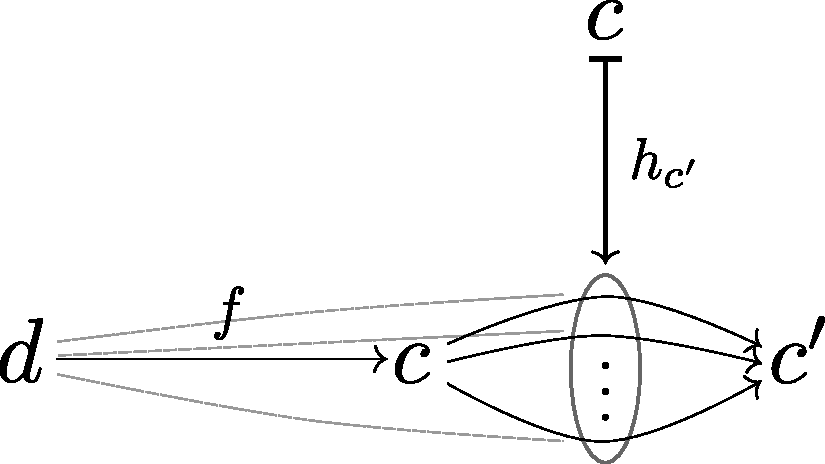
\includegraphics[width=0.7\columnwidth]{fig/hom.pdf}
\caption{The presheaf represented by $c' \in \Ob(\cC)$ is $h^{c'} : \cC^{opp} \rightarrow \textit{Sets}$. It sends objects to the set of morphisms in which they are the domain object with codomain $c'$ and morphisms $f:d \rightarrow c \in \Mor{\cC}$ to set functions $h^{c'} \circ f: \Mor_{\cC}(c,c') \rightarrow \Mor_{\cC}(d,c')$ via pre-composition.}
\label{fig:hom}
\end{figure}

The action of $h^c$ on objects and morphisms is summarized in figure \ref{fig:hom}. The preceding definitions are standard category theoretic constructions. Ellerman has proposed an interpretation of adjoint functors, that demonstrates their relevance to the concept of information encoding and decoding (or sending and receiving) in the context of biological systems \cite{Ellerman2005}.

\iftoggle{thmsty}{
\begin{definition}
\label{definition-birepresentable}
}{}
A bifunctor $bif (-,-): \cC^{opp} \times \cD \rightarrow \textit{Sets}$ is said to be {\it birepresentable} if there exists a pair of functors $F:\cC^{opp} \rightleftarrows \cD:G$ where $c \in \Ob(\cC^{opp})$ and $d \in \Ob(\cD)$ gives
\begin{eqnarray*}
b^{d} \equiv bif(-,d) &:& \mathcal{C}^{opp} \rightarrow \textit{Sets},\\
b_{c} \equiv bif(c,-) &:& \mathcal{D} \rightarrow \textit{Sets}.
\end{eqnarray*}
natural in $c$ and $d$ such that $F \dashv G$. The functors $b^{d}$ and $b_{c}$ are defined on
\begin{enumerate}
\item objects for all $c_i \in \Ob(\cC^{opp})$ and for all $d_i \in \Ob(\cD)$
\begin{eqnarray*}
b^{d} (c_i) &=& \Mor_{\cC^{opp}}(c_i,Gd),\\
b_{c} (d_i) &=& \Mor_{\cD}(Fc,d_i).
\end{eqnarray*}

\item morphisms for all $f_{ij}:c_j \rightarrow c_i \in \Mor(\cC^{opp})$ and for all $g_{ij}:d_i \rightarrow d_j \in \Mor(\cD)$ as
\begin{eqnarray*}
b^{d} (f_{ij}) &:& \Mor_{\cC^{opp}}(c_i,Gd) \rightarrow \Mor_{\cC^{opp}}(c_j,Gd),\\
b_{c} (g_{ij}) &:& \Mor_{\cD}(Fc,d_i) \rightarrow \Mor_{\cD}(Fc,d_j).
\end{eqnarray*}
\end{enumerate}
\iftoggle{thmsty}{
\end{definition}
}

$F \dashv G$ is thus equivalent to the statement $\phi_{-,-}:b_{(-)} \cong b^{(-)}$. In this framework, information encoding/decoding is an asymmetric process that can only be accomplished without loss of information in one direction: objects of $\cD$ can be encoded into objects of $\cC$ and decoded into objects of $\cD$ but, in general, proceeding in the opposite order may result in loss of information. This asymmetry is clarified by consideration of the unit and counit morphisms of the adjunction.

\iftoggle{thmsty}{
\begin{definition}
\label{definition-unit}
}{}
Consider the identity morphism $1_{Fc} \in \Mor_{\cD}(Fc,Fc)$. The adjoint transpose of $1_{Fc}$ is the {\it unit} morphism at $c$
$$
\phi_{c,Fc}(1_{Fc})=1_{Fc}^*=\eta_c: c \rightarrow GFc
$$
where $\eta_c \in \Mor_{\cC^{opp}}(c,GFc)$, which, when taken to be natural in $c \in \Ob(\cC^{opp})$, gives the natural transformation
$$
\eta : 1_{\cC^{opp}} \Rightarrow GF
$$
\iftoggle{thmsty}{
\end{definition}
}

\iftoggle{thmsty}{
\begin{definition}
\label{definition-counit}
}{}
Consider the identity morphism $1_{Gd} \in \Mor_{\cC^{opp}}(Gd,Gd)$. The adjoint transpose of $1_{Gd}$ is the {\it counit} morphism at $d$
$$
\phi_{Gd,d}^{-1}(1_{Gd})=1_{Gd}^*=\epsilon_d: FGd \rightarrow d
$$
where $\epsilon_d \in \Mor_{\cD}(d,FGd)$, which, when natural in $d$, gives the natural transformation
$$
\epsilon: FG \Rightarrow 1_{\cD}
$$
\iftoggle{thmsty}{
\end{definition}
}

The composite encoding inspection functor 
$$
b_{(-)} \circ G(-): \cD \rightarrow \cC^{opp} \rightarrow \textit{Sets}
$$
that specifies a set of morphisms in $\cD$ from the perspective of $\cC^{opp}$ is represented by the pair $(F,\eta)$. Likewise, the composite decoding inspection functor 
$$
b^{(-)} \circ F(-): \cC^{opp} \rightarrow \cD \rightarrow \textit{Sets}
$$
that specifies a set of morphisms in $\cC^{opp}$ from the perspective of $\cD$ is represented by the pair $(G,\epsilon)$. Figure \ref{fig:adjunction} summarizes features of the information encoding-decoding adjunction between $F$ and $G$.

\begin{figure}
\noindent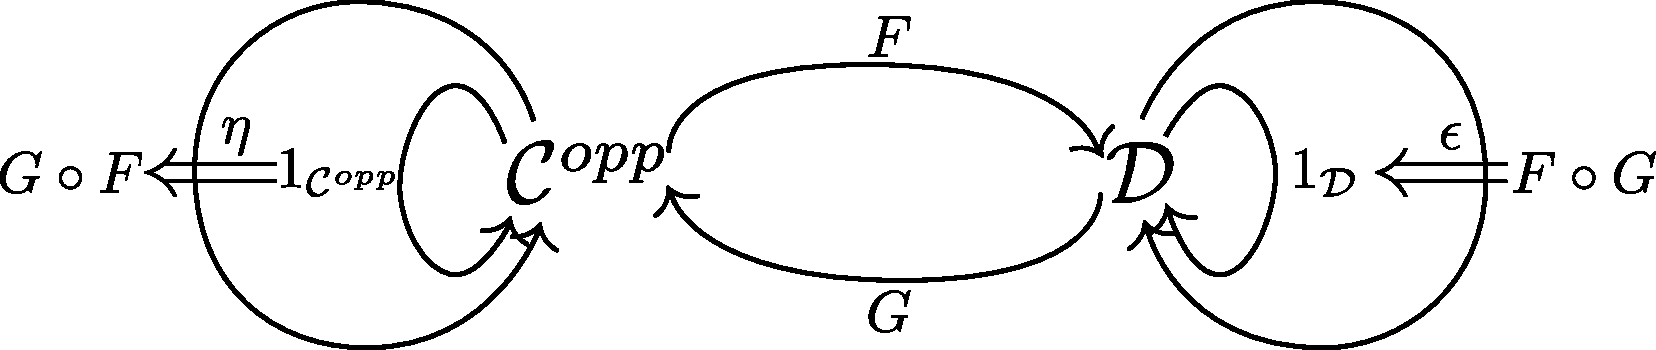
\includegraphics[width=0.9\columnwidth]{fig/adjunction.pdf}
\caption{The adjoint relationship between functors $F \dashv G$ with unit $\eta$ and counit $\epsilon$ natural transformations. The asymmetry in the encoding-decoding relationship indicates that $FG \cD$ can be translated back into the original terms of $\cD$ whereas $GF \cC^{opp}$ cannot be translated back into the original terms of $\cC^{opp}$.}
\label{fig:adjunction}
\end{figure}

The asymmetry of the adjunction can be dispensed with if the unit and counit natural transformations are in fact natural isomorphisms $\eta: 1_{\cC^{opp}} \cong GF$ and $\epsilon: FG \cong 1_{\cD}$. In any limit in which this is the case the adjunction $F \dashv G$ gives an equivalence of categories $\cC^{opp} = \cD$ and the information encoding-decoding process becomes bidirectionally exact.

\subsection{Intrinsic measurement processes of biological systems}
The perspective taken here seeks to abstract from the fundamental relationship between algebraic structures and geometric state spaces that enables translation between them in certain cases \cite{Nestruev2002}. The significance of this perspective is in its capacity to address an important issue that arises in the process of constructing models of biological systems. It is conventional to assume that the geometry of the state space in dynamical models of biological systems is invariantly Euclidean leading to the specification of models of biological systems as a system of ordinary differential equations or the flow of a vector field on a Euclidean manifold, colloquially written as something similar to
$$
\frac{d \vec{x}}{dt} = V(\vec{x}),
$$ 
where $\vec{x}$ is a vector of state variables upon which $V$ is a function specifying a vector field that, for each variable, may be a function of all specified state variables. This framework requires generalization to approach accurate representation of biological systems, which are evolvable. Presumably, the geometry of the state space is not fixed {\it a priori} and is itself constructed as part of the intrinsic dynamics intuitively associated to current understanding of biological systems \cite{Fontana1994,Fontana1996}. In this light, we need to explicitly consider the process by which a state space is intrinsically constructed in the context of developing a theoretical framework for constructing models of biological systems. This can be accomplished within an {\it intrinsic operational framework} that begins with an abstract accounting of measurements that biological entities may perform upon one another leading to the view of morphisms in a category as specifying a measurement process in which the structure of a biological entity is measured in terms of the structure of another \cite{Rosen1978}.
 
At any level of organization, for example in the case of protein-protein interactions \cite{Johnson2010a, Heo2011}, there are interactions that do not provide stable channels for information flow or may poison otherwise stable channels resulting in the appearance of fundamental randomness at the population level. At another extreme, interactions that do support information flow at the population level are robust correlations that may in turn impinge as a selective filter for a particular type of information flow in another connected, but potentially distal, interaction. The space spanning these relative extremes is embodied in structure preserving transformations between objects in a category where the domain object is viewed as an observable and the codomain object is viewed as representing the result of an intrinsic measurement. Of course, these objects may themselves be represented by categories or some higher-order algebraic structure in which the notion of structure preservation implies important subtleties, but the interpretation of a process in which observables take values according to measurements is invariant.
From this perspective, what is necessary to characterize any biological entity is precisely a mechanism for determining the set of interactions in which it participates from the point of view of any other entity with which it interacts. This simple principle has a precise formulation in category theory in terms of {\it Yoneda's lemma}.

\iftoggle{thmsty}{
\begin{definition}
\label{lemma-yoneda}
}{}
Given a category $\cC$, for $c,c' \in \Ob(\cC)$ and $h_{c},h_{c'} \in \Ob(\textit{Sets}^{\cC})$, the {\it covariant Yoneda lemma} states that the set of natural transformations between copresheaves $Nat_{\textit{Sets}^{\cC}}(h_{c'},h_c)$ is isomorphic to $h_{c}(c')=Mor_{\cC}(c,c')$ and natural in $c$ and $c'$:
$$
Nat_{\textit{Sets}^{\cC}}(h_{c'},h_c) \cong Mor_{\cC}(c,c')
$$
Dually, for $h^{c},h^{c'} \in \Ob(\textit{Sets}^{\cC^{opp}})$ the {\it contravariant Yoneda lemma} states that the set of natural transformations between presheaves $Nat_{\textit{Sets}^{\cC^{opp}}}(h^{c},h^{c'})$ is isomorphic to $h^{c'}(c)=Mor_{\cC^{opp}}(c,c')$ and natural in $c$ and $c'$:
$$
Nat_{\textit{Sets}^{\cC^{opp}}}(h^{c},h^{c'}) \cong Mor_{\cC^{opp}}(c,c')
$$
\iftoggle{thmsty}{
\end{definition}
}

The covariant form of Yoneda's lemma in the reverse direction from morphisms to natural transformations implies that if we have an intrinsic measurement procedure $f:c \rightarrow c' \in Mor(\cC)$  where an observable $c$ takes values in $c'$ as the result of an interaction between $c$ and $c'$ then we have an associated natural transformation between the functors represented by $c'$ and $c$, $\xi^{c'}_{c} : h_{c'} \Rightarrow h_c$. 
This relationship has two important meanings. The first is that all of the information implicit in a particular biological entity can be expressed in terms of the set of intrinsic measurement procedures to which it is subjected in interactions with all other biological entities, which is formalized in terms of the functor that it represents $h_c \equiv hom(c,-)$, being a variable set of morphisms parametrized by all other biological entities within the category of such. The second is that if two biological entities interact with all others in equivalent ways, then this will be identified according to the Yoneda lemma by the existence of a natural isomorphism between the functors represented by each.

Depending upon the specific nature of the category modelling biological entities, the functor $h_c$ can be endowed with a geometric interpretation. For example, the evaluation of $h_c$ from the perspective of any $c' \in \Ob(\cC)$ can be taken to represent the set of states within a geometric space that represent $c$ in terms of $c'$ under all possible measurement procedures acting on $c$. Dually, evaluation of the functor $h^c$ from the perspective of any $c' \in \Ob(\cC)$ can be taken to determine all the points specifying measurement values in terms of $c$ which together determine the structure of the state space represented by $c$. In cases where the objects of such a category have sufficient structure, the intuitive security provided by the association between geometry and visualizability is illusory because the only known methods of interrogation of such complicated objects are algebraic. The geometric semantics are nevertheless helpful in the context of explaining the modelling framework.

\subsection{Topological features of biological information representation}



\subsection{Variable filtration of biological information}

\subsection{Deconstructing and synthesizing biological information}

\subsection{Enabling conditions of hierarchical transformations}

\section*{Acknowledgements} 

a1 was supported by . 
a2 was supported by .
a3 was supported by .
a4 was supported by .

%-----------------------------------------------%
%                   appendix
%-----------------------------------------------%
\appendix
\section{Category theory for tourists}


%------bibliography---%
\bibliographystyle{unsrt} 
\bibliography{bib/books,bib/papers}
%---------------------%

\end{document}